% Created 2022-05-19 Thu 14:47
% Intended LaTeX compiler: pdflatex
\documentclass{article}
\usepackage[utf8]{inputenc}
\usepackage[T1]{fontenc}
\usepackage{graphicx}
\usepackage{longtable}
\usepackage{wrapfig}
\usepackage{rotating}
\usepackage[normalem]{ulem}
\usepackage{amsmath}
\usepackage{amssymb}
\usepackage{capt-of}
\usepackage{hyperref}
\usepackage[cachedir=/tmp/minted]{minted}
\usepackage{color}
\usepackage{tikz}
\usepackage{fancyvrb}
\usepackage[a4paper]{anysize}
\usepackage{minted}
\usepackage{xparse}
\usepackage{forest}

\renewcommand{\labelenumii}{\arabic{enumi}.\arabic{enumii}}
\renewcommand{\labelenumiii}{\arabic{enumi}.\arabic{enumii}.\arabic{enumiii}}
\renewcommand{\labelenumiv}{\arabic{enumi}.\arabic{enumii}.\arabic{enumiii}.\arabic{enumiv}}


\newminted{c}{tabsize=4,obeytabs,autogobble,highlightcolor=gray!20}
\newenvironment{env}{\VerbatimEnvironment\begin{ccode}}{\end{ccode}}
\newmintinline{c}{}
\newmintedfile{c}{tabsize=4,obeytabs,linenos,frame=single,highlightcolor=gray!50}
\setcounter{secnumdepth}{4}
\author{Isak Mikaelsson (\texttt{tfy20imn@cs.umu.se})\\
Henrik Linder (\texttt{tfy18hlr@cs.umu.se})
}
\date{\today}
\title{5DV149 LP4 --- Assignment 4\\\medskip
\large Graphs\\
Submission v1.0}
\begin{document}
\maketitle
\clearpage \tableofcontents \clearpage\addtocounter{section}{-1}
\section{Version history}
\label{sec:history}
\begin{description}
\item[{v1.0 \today}] First submission.\footnote{If this is a resubmission, 
include a list of changes with
respect to the previous submission.}
\end{description}
\section{Introduction}
\label{sec:intro}
The graph is a data type consisting of nodes and edges connecting these nodes. Graphs have many applications as for example models for electric circuits, or describing networks of different kinds. These networks could for example be describing street maps, communication networks, or travel routes. The last kind is the one we have worked with in this lab. 
In this assignment, we set out to read in information about available flight routes between different airports in Sweden, stored in text files, and convert this information to a graph of available flights. Then we wrote a program that used this graph to determine whether there is a path to get from one airport to another. 
An example of a graph to be can be seen in \ref{fig:graph2} below. 

In order to determine whether there is a path between two nodes, a breadth-first algorithm was implemented, traversing the graph from the start node until the destination node is found, or until all nodes connected to the start node has been checked. 

% \textcolor{red}{The target audience is someone with basic understanding in Computing
% Science, but not specifically graphs nor the application, e.g., a
% future colleague at your work who did not take part in this particular
% project. Describe the application and how it connects to graphs. You
% may include a figure, e.g. as in figures \ref{fig:graph1} and \ref{fig:graph2}.}
% \begin{figure}[tbp]
% \centering
% \includegraphics[width=0.2\hsize]{graph1.png}
% \caption{\label{fig:graph1}Graph illustration corresponding to the file \
% texttt{airmap1.map}, png version.}
% \end{figure}
\begin{figure}[H]
  \begin{center}
    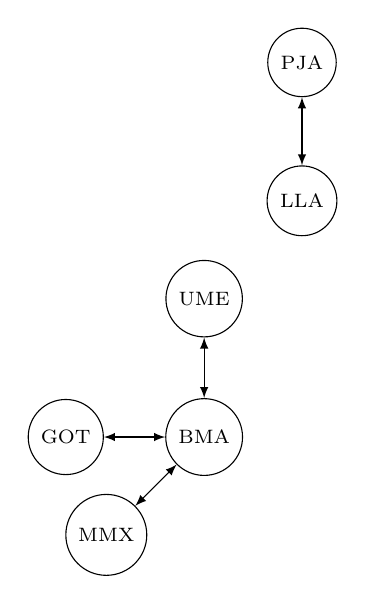
\begin{tikzpicture}[node distance=5em,font=\scriptsize]
      \node[draw,circle] (ume) { UME };
      \node[draw,circle,below of=ume] (bma) { BMA };
      \node[draw,circle,below left of=bma] (mmx) { MMX };
      \node[draw,circle,left of=bma] (got) { GOT };
      \node[draw,circle,above right of=ume] (lla) { LLA };
      \node[draw,circle,above of=lla] (pja) { PJA };
      \draw[latex-latex] (ume) -- (bma);
      \draw[latex-latex] (mmx) -- (bma);
      \draw[latex-latex] (got) -- (bma);
      \draw[latex-latex] (lla) -- (pja);
    \end{tikzpicture}
  \end{center}
\caption{\label{fig:graph2}Graph illustration corresponding to the file \texttt{airmap1.map}.}
\end{figure}



\section{User guide}
\label{sec:user_guide}
\subsection{Compilation}
\label{sec:compilation}
% \textcolor{red}{ Describe exactly how the reader might compile the code, assuming
% he/she has access to the source code, e.g.}


\begin{figure}[H]
\begin{forest}
  for tree={
    font=\ttfamily,
    grow'=0,
    child anchor=west,
    parent anchor=south,
    anchor=west,
    calign=first,
    edge path={
      \noexpand\path [draw, \forestoption{edge}]
      (!u.south west) +(7.5pt,0) |- node[fill,inner sep=1.25pt] {} (.child anchor)\forestoption{edge label};
    },
    before typesetting nodes={
      if n=1
        {insert before={[,phantom]}}
        {}
    },
    fit=band,
    before computing xy={l=15pt},
  }
[project root
  [datastructures-v1.0.9
  ]
  [code-folder
    [graph.c]
    [is\_connected.c]
  ]
]
\end{forest}
\caption{\label{fig:file_tree}The file tree for the example compilation.}
\end{figure}
Assuming the user has the code base in the project's root folder and our code in a separate sub-folder, as shown in Fig.\eqref{fig:file_tree} above, the project can be compiled on a Unix-like system by running the following commands. 

\phantomsection
\label{example:compile}
\begin{verbatim}
gcc graph.c -o graph.o -std=c99 -Wall -g -I ../datastructures-v1.0.9/include/ 
\end{verbatim}
\begin{verbatim}
gcc is_connected.c -o is_connected -std=c99 -Wall -g -I ../datastructures-v1.0.9/include/ 
../datastructures-v1.0.9/src/queue/queue.o ../datastructures-v1.0.9/src/dlist/dlist.o
../datastructures-v1.0.9/src/list/list.o graph.o
\end{verbatim}
\subsection{File format}
\label{sec:file_format}
The file containing the graph description is formatted as follows. 

\begin{itemize}
\item The file may contain blank lines or comment lines, starting with \texttt{\#}.

\item The first line that isn't blank or a comment contains an integer denoting the number of edges in the graph. 

\item All other lines each contain one edge:

\item The lines contain two node names separated by whitespaces.

\item There may be whitespaces at the start or end of the lines, in which case they should be ignored.

\item The lines may have comments at the end which should be ignored. 

\item The node names are alphanumerical and are a maximum of 40 characters each. 

\item The final line of the file may be missing a line break. 

\item The text file may be in unix- or dos-format. 

\item There are no duplicate edges in the file. 
\end{itemize}
An example of a file can be seen below. This file was given as an example in the assignment, and is the one shown in Fig.\eqref{fig:graph2} and the one used in the test run in Fig.\eqref{fig:testrun}

% \textcolor{red}{Describe t?he file format.  example : }
\begin{verbatim}
# Some airline network
8
UME BMA # Umea-Bromma
BMA UME # Bromma-Umea
BMA MMX # Bromma-Malmo
MMX BMA # Malmo-Bromma
BMA GOT # Bromma-Goteborg
GOT BMA # Goteborg-Bromma
LLA PJA # Lulea-Pajala
PJA LLA # Pajala-Lulea
\end{verbatim}
\subsection{Test runs}
\label{sec:test_run}
Below is a description of a test run of the finished program. \texttt{is\_connected} is run with the file containing the graph as argument. Then several pairs of start and destination nodes are tested. First, three pairs of nodes where there are paths, including one where the start and destination nodes are the same. 

Then, a few examples of paths and nodes that do not exist. Then the user writes \texttt{quit} for a normal exit.  
\begin{figure}[H]
    \centering
    \includegraphics[width = .7\linewidth]{figs/fulltestrun_bettercrop.png}
    \caption{A test run of the program with the graph file airmap1.map. The user has tested several pairs of airports with existing paths, non-existing paths, and invalid inputs. }
    \label{fig:testrun}
\end{figure}


% \begin{figure}[H]
%     \centering
%     \includegraphics[width = \linewidth]{figs/doenstwork.png}
%     \caption{Caption}
%     \label{fig:not_working_testrun}
% \end{figure}

% \textcolor{red}{ Describe a complete test run, i.e., how the program is started, input
% and output. Screen dumps can be useful here, but be sure to trim them
% to the terminal window where the program is run.}
\section{System description}
\label{sec:system_description}
\subsection{Data structures}
\label{sec:org6e002c6}
\subsubsection{Graph}
\label{sec:graph}
The graph is implemented as a list, and the interface of the implementation is described below.         \\

\noindent
The function \texttt{graph\_empty()} allocates memory for the graph and creates an empty list for the nodes. \\

\noindent
The function \texttt{graph\_is\_empty()} calls the \texttt{dlist}-function \texttt{dlist\_is\_empty} with the list of nodes.\\

\noindent
The function \texttt{graph\_has\_edges(g)} iterates through the list of nodes for the graph \textit{g} and reads a node at each iteration. The read node's neighbours are sent to the \texttt{dlist}-function \texttt{dlist\_is\_empty} to determine whether the list is empty. If the list is not empty, that means that there is an edge, and the function returns 1. If no edge is found in any of the nodes, the function returns 0.\\

\noindent
The function \texttt{graph\_insert\_node(s, g)} allocates memory for a node. The string \textit{s} is then written to the node's \texttt{identifier}, its \texttt{seen\_status} is set to false, and memory is allocated for a potential list of neighbours. Then, a node is inserted into the graph \textit{g} using \texttt{dlist\_insert} and the graph is returned. \\

\noindent
The function \texttt{graph\_find\_node(s, g)} iterates through the list of nodes and reads a node at eaach iteration. The read node's  \texttt{identifier} is compared to \textit{s} using the built-in C-function \texttt{strcmp}. If \texttt{strcmp} returns \texttt{true}, the inspected node is returned. If no \textit{s} matches the identifier of any node, the function returns \texttt{NULL}.\\

\noindent
The function \texttt{graph\_node\_is\_seen(v, g)} returns \texttt{seen\_status} for the node \textit{v}. \\

\noindent
The function \texttt{graph\_node\_set\_seen(v, g, seen)} changes \texttt{seen\_status} for the node \textit{v} to \texttt{seen} and returns the graph \textit{g}. \\

\noindent
The function \texttt{graph\_reset\_seen(g)} iterates through the entire graph \textit{g}, uses \texttt{dlist\_is\_empty} to read each node, and sets its \texttt{seen\_status} to 0. It finally returns the graph \textit{g}. \\

\noindent
The function \texttt{graph\_insert\_edge(n1, n2, g)} starts by reading the list of neighbours for \textit{n1} and the node name \textit{identifier} for \textit{n2}. Then the node name is inserted into the list of neighbours and the updated graph \textit{g} is returned. \\

\noindent
The function \texttt{graph\_delete\_node(v, g)} iterates through the graph \textit{g} and reads nodes that are then compared to \textit{v} through the function \texttt{nodes\_are\_equal}. If the nodes are equal, the node is removed from the list of nodes and the memory from both the node and its list of neighbours is returned. The graph \textit{g} is then returned. \\

\noindent
The function \texttt{graph\_choose\_node(g)} reads and then returns the node tat is at the top of the list of nodes for \textit{g}. \\

\noindent
The function \texttt{graph\_neighbours(n, g)} starts by creating an empty list with \texttt{dist\_empty} and reads the list of neighbours for \textit{n}. Then the function iterates over the list of neighbours and fetches the node for each neighbour with \texttt{graph\_find\_node}. It then rewrites the the empty list with this list. When the nodes for each neighbour have been written to the new list, the list is returned. The memory is not freed by the function but must be freed by the user. \\

\noindent
The function \texttt{graph\_kill(g)} iterates through the list of nodes and at each iteration reads the top node with \texttt{graph\_choose\_node}. This node is then deleted with \texttt{graph\_delete\_node}. Finally, the list is deleted with \texttt{dlist\_kill} and the memory for \textit{g} is freed.

% \textcolor{red}{The graph data structure is central to this assignment. Describe how
% you have designed and implemented the data structure. What information
% is stored and where? If you use a \texttt{struct}, you should probably
% describe it and its fields. How is the allocate/deallocate
% responsibility handled. What help data structures have you used? How
% have you defined equality between nodes? How do you handle (avoid?)
% node duplicate in the graph?
% Describe each function in the interface to the data type \texttt{Graph}. Each
% implemented function should be described in some detail, e.g., input,
% output, actions and any side effects. The interface should be
% organised to be easy to read, e.g., in a table or a bullet list. It is
% ok to include the function declaration, e.g.,}\footnote{If you use latex and minted 
% for this kind of color-coding
% of source code you must probably need to compile the .tex file with
% \texttt{pdflatex -shell-escape file.tex}.}
% \begin{ccode}
% graph *graph_insert_edge(graph *g, node *n1, node *n2);
% \end{ccode}
% \textcolor{red}{but in the text you should refer to \emph{the graph \texttt{g}}, \emph{the node \
% texttt{n1}},
% etc. Never use \texttt{*} in the text. Instead, if it is necessary, write
% ''pointer to\ldots{}''.
% You may group and the unimplemented functions separately. The
% unimplemented function do not need to be described nor commented, only
% listed.}

\subsubsection{Other data structures}
\label{sec:other_data_structures}
% \textbf{dlist}
% The interface for the data type
Beyond graph, we also used the data type doubly linked linked list, \texttt{dlist}, the interface of which can be seen in the table below. 

\begin{table}[H]
\caption{\label{tab:dlist}
A table showing the user interface for the \texttt{dlist} data type.
}
\centering
\begin{tabular}{l|l}
\textbf{Function} & Description\\
\hline
\texttt{dlist\_empty(free\_func)} & Constructs an empty list. \\
\texttt{dlist\_is\_empty(l)} & Returns \texttt{true} if list \textit{l} is empty. \\
\texttt{dlist(l)} & Returns the first position in the list \textit{l} \\
\texttt{dlist\_next(l, p)} & Takes the position \textit{p} and returns the next value in the list \textit{l}. \\
\texttt{dlist\_is\_end(l, p)} & Checks if position \textit{p} is the last element of the list \textit{l} \\
&     and returns \texttt{true} if it is.  \\
\texttt{dlist\_inspect(l, p)} & Returns the value at position \textit{p} in the list \textit{l}. \\
\texttt{dlist\_insert(l, v, p)} &Inserts the value \textit{v} at position \textit{p} in the list \textit{l}. \\
\texttt{dlist\_remove(l, p)} & Removes the value at position \textit{p} in the list \textit{l}. \\
\texttt{dlist\_kill(l)} & Destroys the list \textit{l} and returns all dynamic memory from \\
&the list and its elements.\\
\texttt{dlist\_print(l, print\_func)} & Iterates over the elements in the list \textit{l} and prints their values. \\
\end{tabular}
\end{table}




We also used the data type \texttt{queue}, the interface of which can be seen in the table below. 
% \textbf{queue}
\begin{table}[H]
\caption{\label{tab:queue}
A table showing the user interface for the \texttt{queue} data type.
}
\centering
\begin{tabular}{l|l}
\textbf{Function} & Description\\
\hline
\texttt{queue\_empty(free\_func)} & Constructs an empty queue. \\
\texttt{dlist\_is\_empty(q)} & Returns \texttt{true} if queue \textit{q} is empty. \\
\texttt{queue\_enqueue(q, v)} & Inserts a value \textit{v} into the queue \textit{q}.\\
\texttt{queue\_dequeue(q)} & Removes the first value from the queue \textit{q}.\\
\texttt{queue\_front(q)} & Returns the first value in the queue \textit{q}.\\
\texttt{queue\_kill(q)} & Destroys the queue \textit{q} and returns the memory from\\
&the queue and its elements.\\
\texttt{queue\_print(q, print\_func)} & Prints the values of all elements in the queue \textit{q}. \\
\end{tabular}
\end{table}


% \textcolor{red}{ For each data type from the code base that you have used, e.g.,
% \texttt{queue}, describe it in a separate subsection. In each section,
% describe the datatype briefly in one or a few sentences and then list
% all functions in the user interface. Only make references to
% \emph{published} information about the data type. That includes what is
% known from the header files but not the source.}
\subsection{Algorithms}
\label{sec:algorithms}
\subsubsection{Parsing file}

The algorithm we used for parsing the text files containing the map and generating a graph from the content can be seen in the list below. 
\begin{enumerate}
    \item For each line
    \begin{enumerate}
        \item If line is blank or comment
        \begin{enumerate}
            \item Skip to next line
        \end{enumerate}
        \item If first non-commented line is not an integer
        \begin{enumerate}
            \item Exit with error
        \end{enumerate}
        \item Read number of edges from first line
        \item Remove trailing comments
        \item Remove trailing and preceding whitespaces around the string
        \item Get position of whitespace in string
        \item Save string up to whitespace in array of start node names
        \item Save string after whitespace in array of destination node names
    \end{enumerate}
    \item Create empty graph
    \item For number of edges
    \begin{enumerate}
        \item If start or end node for this edge is not in the graph already
        \begin{enumerate}
            \item Insert that node into the graph
        \end{enumerate}
        \item Get start and destination node for this edge from the graph
        \item If neither of the nodes are \texttt{NULL}
        \begin{enumerate}
            \item Insert an edge between the nodes
        \end{enumerate}
    \end{enumerate}
\end{enumerate}


% \textcolor{red}{ All algorithms must be described in \emph{psedocode}. You may use text to
% summarize the algorithm, but each step must be in some form of
% bulleted or enumerated list. Remember to use variable names, etc., to
% make the algorithm more specific, e.g., ''the current node \(n\)'', etc.}
% \subsubsection{Parsing the text file and constructing the graph}
% \label{sec:parse}
% \textcolor{red}{ Describe your algorithm for parsing the text file and constructing the
% graph. Depending on your implementation, this may be one algorithm or
% two separate ones. You do not have to describe the parsing of each
% line in detail.}
\subsubsection{\texttt{find\_path}}
\label{sec:find_path}
The function \texttt{find\_path} is our implementation of a breadth-first search in the graph to find the destination node. The algorithm we used for this is shown below. 
\begin{enumerate}
    \item While queue of neighbours is not empty
    \begin{enumerate}
        \item Read the top node in the queue
        \item If inspected node is equal to destination node
        \begin{enumerate}
            \item Return 1
        \end{enumerate}
        \item Remove inspected node from queue
        \item Read list of neighbours from inspected node
        \item For each entry in list of neighbours
        \begin{enumerate}
            \item If inspected node is not seen
            \begin{enumerate}
                \item Mark the node as seen and add to queue
            \end{enumerate}
        \end{enumerate}
        \item Free memory for list of neighbours
    \end{enumerate}
    \item Free memory for queue
    \item Reset seen-status for all nodes
    \item Return 0
\end{enumerate}

% \textcolor{red}{ Describe your version of the breadth-first-algorithm that you have
% implemented in \texttt{find\_path}.}
\section{Reflections}
\label{sec:orgd37f281}
\subsection{Work distribution}
\label{sec:org66520d9}
When working on this project, we wanted to make sure that both of us understand the whole of the work process. This includes writing the code and writing the report. Therefore we sat together and did most of the development and design of the algorithm. When we worked individually, we made sure to sit down afterwards and step through the work to make sure that we were both on board with how everything worked. This had the added benefit of making sure that we both had a good enough understanding of the code to be able to help each other when we had issues. 



% \textcolor{red}{ If you worked in groups, how has the work been distributed. How have
% you made sure that everyone understands each part, including parts
% that have been the resposibility of others?}
\subsection{Reflections}
\label{sec:org2c6da4f}
When doing this assignment we found it very interesting to build the graph and particularly to design the algorithms and uses of the code. We spent quite a bit of time at the start of the project sitting down at a whiteboard and sketching different solutions, trying to figure out ways to get everything to behave according to the specifications. In this phase we collaborated a lot with other groups and people that have taken the course previously, which helped in getting different perspectives and fairly quick solutions to the issues that came up along the way. 

This was a surprisingly fun way to get a grip of the assignment and probably saved us some time later since we had a (somewhat) working algorithm from the start and so didn't have to do any major reworkings afterwards. Instead we could just do minor tweaks to account for edge cases that we hadn't considered in the brainstorming phase. 

Overall, the work was fairly painless. Of course, there was the usual amount of swearing over memory leaks and pointers behaving unexpectedly, but no huge bumps on the road. The assignment  was still time consuming and far from trivially simple, but we agree that it turned out fairly well considering the circumstances. 

We both agree that this has been very rewarding work assignment that helped us develop our skills in software development and problem solving much more than the previous assignments. The fact that we had to sit down and plan the structure of the code beforehand was very helpful and forced us to think more in detail about the algorithms, which turned out to be a great experience. 


% \textcolor{red}{ Reflect on the assignment! Did you find anything fun, challenging,
% surprising, frustrating, rewarding, etc. If you submit for a group,
% you may write one reflection for each group member, or one for the whole group.}
% \subsection{Future work (optional)}
% \label{sec:org2c448d8}
% Did you think of anything interesting to try that you did not have
% time to include? If yes, this is the place to present it.
% \clearpage\appendix
% \section{Useful \LaTeX{} examples}
% \label{app:useful-latex-examples}
% Stuff that may be important to some readers, but not all, may be
% deferred to an appendix. The same is true for lengthy material that
% would disrupt the flow of the document if placed immediately where it
% is first referenced. Examples include code listings, file formats,
% standards, complete tables of all experiments, etc.
% \subsection{Figures}
% \label{app:figures}
% Figure \ref{fig:image} shows an example of a figure. Exactly \emph{where} (at top
% or bottom of a page, on a separate page, or ''here'' in the text) to
% put figures/tables is a matter of style. The author of this document
% is of the opinion that ''here'' should be avoided at all cost. It
% might seem advantageous to have the figure close to the text that
% describes it. However, the figure/table should be as self-contained as
% possible. In general, it should be possible to read and understand the
% body text \emph{without} having to look at the figure. Thus, if you are
% forced to write the body text and present the figure such that they
% will work independently, your report and writing style will benefit.
% As the placement of figures and other floats in \LaTeX{} may shift due to
% changes in text, you are encouraged to leave the fine-tuning of image
% placement \textbf{until your document is complete}.
% \begin{figure}[tbp]
% \centering
% \includegraphics[width=0.7\hsize]{./camwithimage8.jpg}
% \caption{\label{fig:image}A figure/image caption should provide sufficient 
% information to make the figure/image as self-explanatory as possible. The caption 
% should be placed under the figure. The latex source shows how to include an image 
% file into a latex document.}
% \end{figure}
% \subsection{Tables}
% \label{app:tables}
% Tables are often used to present tabulated (no sh*t, sherlock?) data
% about the experiment setup, test data, etc., or with results of the
% experiments. In the former case, the body text would typically
% describe what is common with the data sets and then refer to a table
% with detailed information. In the latter case, do not discuss the
% structure of the table in the body text! That would just confuse the
% reader. Such information belongs to the caption. In general, do not
% refer to the table such that the reader cannot continue without
% inspecting the table. Instead, summarize enough of the content of the
% table to allow the reader to continue to the next paragraph.
% Data that can better be summarized in the body text should so appear,
% e.g., ''The execution time for experiment x was below 2ms. The other
% execution times are given in Table x.''
% In all cases, consider the number of significant digits! Do not put a
% gazillion decimals in your tables just because your code spits it out!
% Make the table as easy to read as possible. An example of a stub of a
% results table is given in Table \ref{tab:time-table}.
% \begin{table}[tbp]
% \caption{\label{tab:time-table}A table caption should provide information that 
% helps the reader to understand what data is in the table. Some additional 
% information, e.g., units can also be part of the caption. A table caption should be
% placed above the table proper. Use as few borders in the table as possible! For 
% instance, adding left and right borders to the table below would make it harder to 
% read.}
% \centering
% \begin{tabular}{l|l}
% \textbf{Table type} & Lookup speed (ms)\\
% \hline
% MTFTable & x\\
% Arraytable & y\\
% DListTable & z\\
% \end{tabular}
% \end{table}
\end{document}
